\scanpage{65}
% L01-04, top relations
\[\sigma_0\quad\sigma_1\quad\sigma_2\]
\[r=(s_0,a_0,f_0)\]
\[
\begin{aligned}
\sigma_0s_0&=s_1&\sigma_0a_0&=a_0&\sigma_0f_0&=f_0\\
\sigma_1s_0&=s_0&\sigma_1a_0&=\{s_0,s_2\}&\sigma_1f_0&=f_0\\
\sigma_2s_0&=s_0&\sigma_2a_0&=a_0&\sigma_2f_0&=\{s_0,s_1,s_3\ldots\}
\end{aligned}
\qquad
\begin{aligned}a_0&=\{s_0,s_1\}\\f_0&=\{s_0,s_1,s_2\ldots\}\end{aligned}
\]
% L05-07, left of main drawing
\[\begin{aligned}\sigma_0s_0&=s_1\\\sigma_1s_1&=s_2\\\sigma_2s_2&=s_3\end{aligned}\]
% Main drawing
% crop-candidate: scan 65
\figure{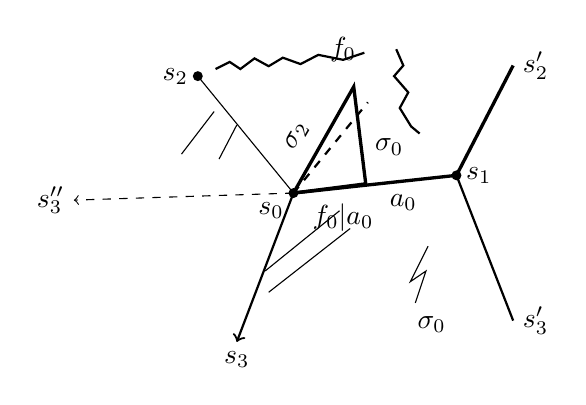
\begin{tikzpicture}[scale=.9]
\coordinate (s0) at (0,0); \coordinate (s1) at (2.3,.25);
\coordinate (s2) at (-1.35,1.65); \coordinate (s3) at (-.8,-2.1);
\coordinate (s2p) at (3.1,1.8); \coordinate (s3p) at (3.1,-1.8);
\draw (s2)--(s0); \draw[thick,->] (s0)--(s3);
\draw[very thick] (s0)--(s1)--(s2p); \draw[thick] (s1)--(s3p);
\draw[->,dashed] (s0)--(-3.1,-.1);
\draw[very thick] (s0)--(.85,1.5)--(1.02,.13)--cycle;
\draw[dashed,thick] (s0)--(1.05,1.28);
\draw[thin] (-1.58,.55)--(-1.12,1.15); \draw[thin] (-1.05,.48)--(-.8,.96);
\draw[thin] (-.4,-1.1)--(.65,-.25); \draw[thin] (-.35,-1.4)--(.8,-.5);
\draw[thick] (-1.1,1.75)--(-.9,1.85)--(-.75,1.75)--(-.55,1.9)--(-.35,1.79)--(-.15,1.91)--(.1,1.82)--(.35,1.95)--(.7,1.88)--(1,1.98);
\draw[thick] (1.45,2.03)--(1.55,1.8)--(1.42,1.65)--(1.62,1.42)--(1.5,1.2)--(1.66,.94)--(1.78,.84);
\draw (1.9,-.75)--(1.65,-1.25)--(1.87,-1.1)--(1.72,-1.55);
\fill (s2) circle (2pt) (s0) circle (2pt) (s1) circle (2pt);
\node[below left] at (s0) {$s_0$}; \node[right] at (s1) {$s_1$};
\node[left] at (s2) {$s_2$}; \node[below] at (s3) {$s_3$};
\node[right] at (s2p) {$s'_2$}; \node[right] at (s3p) {$s'_3$};
\node[left] at (-3.1,-.1) {$s''_3$};
\node[below] at (1.55,.12) {$a_0$};
\node at (.7,2.03) {$\deleted{\unsure{f_0}}$};
\node[rotate=60] at (.05,.8) {$\unsure{\sigma_2}$};
\node at (1.35,.65) {$\sigma_0$};
\node at (.7,-.35) {$\deleted{\unsure{f_0|a_0}}$};
\node at (1.95,-1.85) {$\unsure{\sigma_0}$};
\end{tikzpicture}}
% L05-07, right of main drawing
\[
\left\{\begin{aligned}e_1&=s_1-s_0\\e_2&=s_2-s_0\\e_3&=s_3-s_0\end{aligned}\right.
\]
% L08-11, three action lists
\[
\sigma_0\left\{\begin{aligned}s_0&\longmapsto s_1\\s_1&\longmapsto s_0\\s_2&\longmapsto s'_2\\s_3&\longmapsto s'_3\end{aligned}\right.
\quad
\sigma_1\left\{\begin{aligned}s_0&\longmapsto s_0\\s_1&\longmapsto s_2\\s_2&\longmapsto s_1\\s_3&\longmapsto s''_3\end{aligned}\right.
\quad
\sigma_2\left\{\begin{aligned}s_0&\longmapsto s_0\\s_1&\longmapsto s_1\\s_2&\longmapsto s_3\\s_3&\longmapsto s_2\end{aligned}\right.
\]
% Isolated cancelled symbol between action lists and plane equalities
\[\deleted{\unsure{\sigma_2}}\]
% L08-11, boxed notes at right
\[
\boxed{\begin{gathered}\mathrm{Pl}(s_0,s_1,s_2)\\\deleted{\unsure{(s_0,s_1,s_0)}}\\=\mathrm{Pl}(s_0,s_1,s'_2)\end{gathered}}
\]
\[\boxed{\mathrm{Pl}(s_0,s_1,s_3)=\mathrm{Pl}(s_0,s_1,s'_3)}\]

% L12-16, commuting relation and comparison table
\diagram{\begin{tikzcd}[ampersand replacement=\&]
\begin{gathered}
\boxed{\sigma_0\sigma_2=\sigma_2\sigma_0}\\
\begin{array}{c|cc}
s_0\mapsto&s_1&s_1\\
s_1\mapsto&s_0&s_0\\
s_2\mapsto&s'_3&\sigma_2s'_2\\
s_3\mapsto&s'_2&\sigma_2s'_3
\end{array}
\end{gathered}\arrow[dr,Leftrightarrow]\&\\
\&\begin{gathered}\boxed{\sigma_2s'_2=s'_3}\\\sigma_2s'_3=s'_2\end{gathered}
\end{tikzcd}}
% L12-14, involution conditions to the right
\diagram{\begin{tikzcd}[ampersand replacement=\&]
\boxed{\sigma_0^2=1}\arrow[dr,Leftrightarrow]\&\\
\&\boxed{\begin{aligned}\sigma_0s'_2&=s_2\\\sigma_0s'_3&=s_3\end{aligned}}
\end{tikzcd}}
\diagram{\begin{tikzcd}[ampersand replacement=\&]
\boxed{\sigma_1^2=1}\arrow[dr,Leftrightarrow]\&\\
\&\boxed{\sigma_1s''_3=s_3}
\end{tikzcd}}
\[\sigma_2^2=1\quad\text{automatique}\]

% L17, linked by the curved double arrow to sigma_2 s'_2=s'_3 above
\diagram{\begin{tikzcd}[ampersand replacement=\&,row sep=small]
{}\arrow[d,bend left=35,Leftrightarrow]\\{}
\end{tikzcd}}
% Coordinate tuples are added above the right ends of the two expressions.
\[
s'_2=s_0+\lambda e_1+\mu e_2\inserted{=(\lambda,\mu,0)}
\qquad s'_3=s_0+\lambda e_1+\mu e_3\inserted{=(\lambda,0,\mu)}
\]
\[
\left[\underbrace{\mu=1}_{?},\ \lambda=1+\beta\ldots\right.
\]
% L18-19
\[
\begin{aligned}
s''_3&=s_3+\xi e_1+\eta e_2+\zeta e_3\\
&=s_0+\xi e_1+\eta e_2+(1+\zeta)e_3=(\xi,\eta,1-\zeta)
\end{aligned}
\]
\[
\left[\underbrace{\unsure{\xi|\zeta}=-\eta}_{?},\ \eta=1+\alpha,\ \underbrace{\zeta=0}_{?}\right.
\]
% Lower-left drawing
\figure{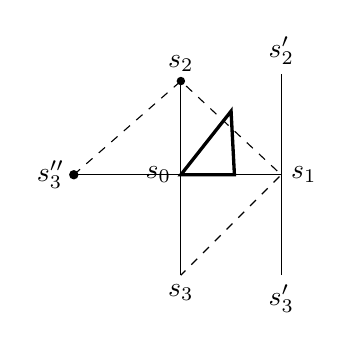
\begin{tikzpicture}[scale=.85]
\draw (0,-1.5)--(0,1.4); \draw (1.5,-1.5)--(1.5,1.5);
\draw (-1.6,0)--(1.5,0);
\draw[dashed] (-1.6,0)--(0,1.4)--(1.5,0)--(0,-1.5);
\draw[very thick] (0,0)--(.75,.95)--(.8,0)--cycle;
\fill (-1.6,0) circle (2pt) (0,1.4) circle (1.8pt);
\node[left] at (-1.6,0) {$s''_3$}; \node[left] at (0,0) {$s_0$};
\node[above] at (0,1.4) {$s_2$}; \node[below] at (0,-1.5) {$s_3$};
\node[right] at (1.5,0) {$s_1$}; \node[above] at (1.5,1.5) {$s'_2$};
\node[below] at (1.5,-1.5) {$s'_3$};
\end{tikzpicture}}
% L20-23
\[
\left\{\begin{aligned}
\sigma_0s_0&=s_1=(1,0,0)\\
\sigma_0e_{\unsure{0|1}}&=-e_1\\
\sigma_0e_2&=(\lambda-1)e_1+\mu e_2\\
\sigma_0e_3&=(\lambda-1)e_1+\mu e_3
\end{aligned}\right.
\]
% L24
\[
\sigma_0=\begin{pmatrix}
-1&\lambda-1&\lambda-1&1\\
0&\mu&0&0\\
0&0&\mu&0\\
0&0&0&1
\end{pmatrix}
\]
% archive sheet number: 64
